\documentclass[11pt,a4paper,titlepage]{article}
\usepackage{subscript,subfigure,amsmath,amssymb,amstext,amsfonts,mathrsfs,graphicx}

\begin{document}

\title{GEP Protokoll - Laborversuch 6\\[1ex]
Messen transienter Vorg\"ange mit dem Oszilloskop}
\author{Cao Thi Huyen \and Robert R\"osler \and Nico Grimm}
\date{15. Dezember 2015}

\maketitle

\section{Zeitmessung}
Es ist die Ausgangsspannung eines Rechteckgenerators auf dem Oszilloskop darzustellen. Mit Hilfe des men\"ugesteuerten Cursors sind daraus Anstiegs- und Abfallzeiten der Impulse auf der Basis 10\% -- 90\% -- 10\% zu bestimmen.

\begin{figure}[h!]
  \subfigure[Anstiegszeit]{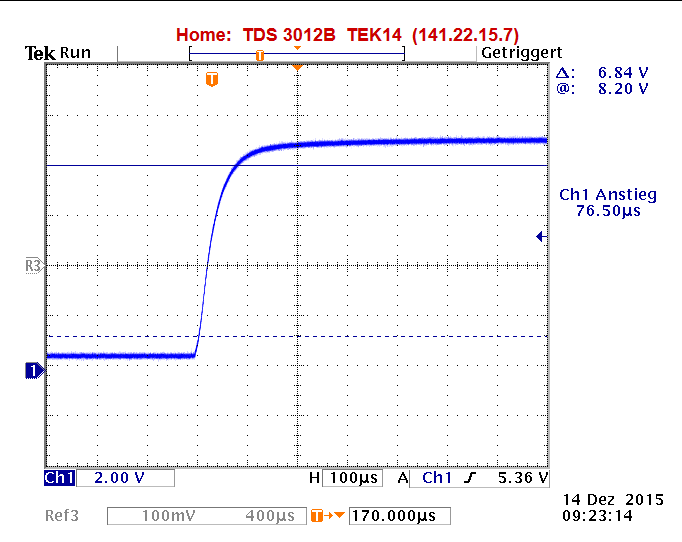
\includegraphics[width=0.49\textwidth]{6-1-auf}}
  \subfigure[Abfallzeit]{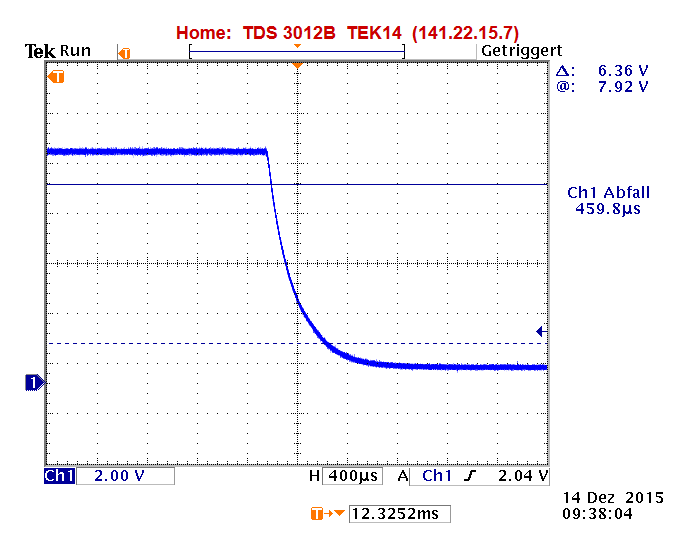
\includegraphics[width=0.49\textwidth]{6-1-ab}}
  \caption{Anstiegszeit: $76.5\mu s$ --- Abfallzeit: $459.8\mu{}s$}
\end{figure}

\subsection{place holder - frequenz \& tastverh\"altnis}
% TO DO

\newpage

\section{Zeit- und Spannungsmessung bei einmaligen Vorg\"angen}

\subsection{Darstellung einmaliger Vorg\"ange: Ein- und Ausschalten eines Relais}
An einem Kammrelais sollen die zeitlichen Verl\"aufe von Strom oder Spannung sowie das Schaltverhalten des Relaisschalters (u\textsubscript{Kont}) \underline{gleichzeitig} dargestellt werden. Da sich die Vorg\"ange im  ms-Bereich abspielen, ist auf eine sichere Triggerung zu achten. \\
Unsere Triggerspannung ist hierbei gr\"o\ss{}er als 2V und unsere Betriebsspannung $u_B=15V$\\[1ex]

\subsubsection{Schaltplan}
\begin{center}
  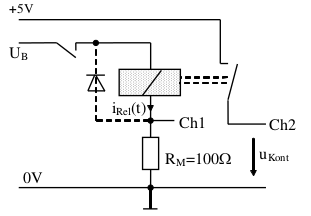
\includegraphics[width=0.7\textwidth]{schaltplan_2_1}
\end{center}

\subsection{Messung 1: Einschaltvorgang}
%TO DO

\newpage

\subsection{Messung 2: Abschaltvorgang}
Nun entfernen wir den Widerstand $R_M$ und messen die Spannung u\textsubscript{Rel}(t) \"uber der Relaisspule. \\
Da beim Abschalten von Induktivit\"aten induzierte Spannungen \textgreater250V auftreten k\"onnen, ist die Benutzung des \textbf{10:1 Tastteiler} zwingend vorgegeben!\\
Wir betrachten hierbei zwei verschiedene Fälle:\\
\begin{itemize}
\item a) ohne \textit{"L\"oschdiode"}
\item b) mit einer L\"oschdiode (IN 4007) zur Vermeidung des Schaltfunkes
\end{itemize}

\begin{figure}[h!]
  \subfigure[Fall a)]{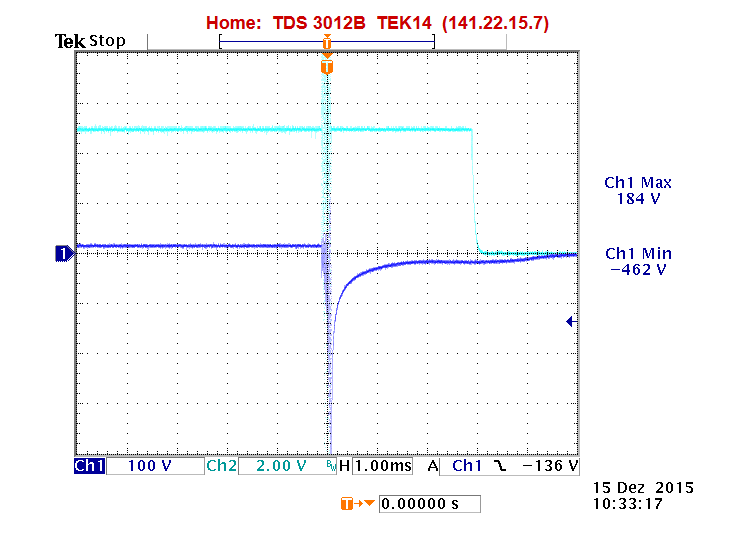
\includegraphics[width=0.49\textwidth]{6-2-2}}
  \subfigure[Fall b)]{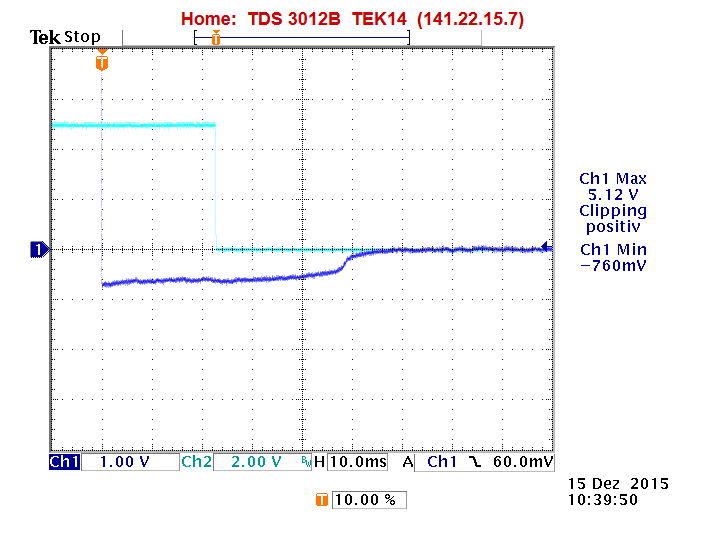
\includegraphics[width=0.49\textwidth]{6-2-3}}
  \caption{Spannung \"uber der Relaisspule}
\end{figure}

\subsubsection*{Fall a: ohne L\"oschdiode}
Gemessen wurde eine Maximalspannung $\hat{u}_{Rel}=462V$ und eine Verz\"ogerungszeit $t_{ab}=3ms$
\subsubsection*{Fall b: mit L\"oschdiode}
Gemessen wurde eine Maximalspannung $\hat{u}_{Rel}=760mV$ und eine Verz\"ogerungszeit $t_{ab}=50ms$

\newpage

\subsection{Darstellung einmaliger Vorg\"ange: Auf- und Entladen eines Kondensators}
Zu folgender Schaltung sind mehrere Aufgabe zu l\"osen.
\begin{figure}[h!]
  \begin{center}
    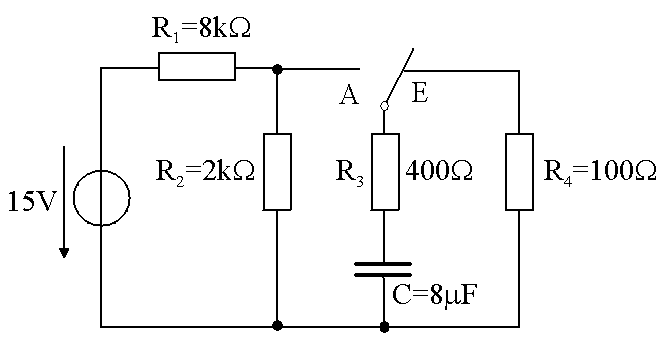
\includegraphics[width=0.7\textwidth]{schaltplan_2_2}
    \caption{Schaltplan}
  \end{center}
\end{figure}

\subsubsection{F\"ur die Umschaltung von E nach A (Aufladung)}
Als Vorausberechnung bestimmen wir die Aufladezeitkonstante $\tau_A$ und die Kondensatorspannung $u_{c, End}$ im aufgeladenen Zustand.

\subsubsection{F\"ur die Umschaltung von A nach E (Entladung)}
Als Vorausberechnung bestimmen wir die Entladezeitkonstante $\tau_E$.

\subsubsection{Zeitlicher Verlauf der Kondensatorspannung}

\subsubsection{Bestimmung von $\tau_A$ und $\tau_E$ anhand des Schirmbildes}

\end{document}
